\documentclass[twoside]{book}

% Packages required by doxygen
\usepackage{fixltx2e}
\usepackage{calc}
\usepackage{doxygen}
\usepackage[export]{adjustbox} % also loads graphicx
\usepackage{graphicx}
\usepackage[utf8]{inputenc}
\usepackage{makeidx}
\usepackage{multicol}
\usepackage{multirow}
\PassOptionsToPackage{warn}{textcomp}
\usepackage{textcomp}
\usepackage[nointegrals]{wasysym}
\usepackage[table]{xcolor}

% Font selection
\usepackage[T1]{fontenc}
\usepackage[scaled=.90]{helvet}
\usepackage{courier}
\usepackage{amssymb}
\usepackage{sectsty}
\renewcommand{\familydefault}{\sfdefault}
\allsectionsfont{%
  \fontseries{bc}\selectfont%
  \color{darkgray}%
}
\renewcommand{\DoxyLabelFont}{%
  \fontseries{bc}\selectfont%
  \color{darkgray}%
}
\newcommand{\+}{\discretionary{\mbox{\scriptsize$\hookleftarrow$}}{}{}}

% Page & text layout
\usepackage{geometry}
\geometry{%
  a4paper,%
  top=2.5cm,%
  bottom=2.5cm,%
  left=2.5cm,%
  right=2.5cm%
}
\tolerance=750
\hfuzz=15pt
\hbadness=750
\setlength{\emergencystretch}{15pt}
\setlength{\parindent}{0cm}
\setlength{\parskip}{0.2cm}
\makeatletter
\renewcommand{\paragraph}{%
  \@startsection{paragraph}{4}{0ex}{-1.0ex}{1.0ex}{%
    \normalfont\normalsize\bfseries\SS@parafont%
  }%
}
\renewcommand{\subparagraph}{%
  \@startsection{subparagraph}{5}{0ex}{-1.0ex}{1.0ex}{%
    \normalfont\normalsize\bfseries\SS@subparafont%
  }%
}
\makeatother

% Headers & footers
\usepackage{fancyhdr}
\pagestyle{fancyplain}
\fancyhead[LE]{\fancyplain{}{\bfseries\thepage}}
\fancyhead[CE]{\fancyplain{}{}}
\fancyhead[RE]{\fancyplain{}{\bfseries\leftmark}}
\fancyhead[LO]{\fancyplain{}{\bfseries\rightmark}}
\fancyhead[CO]{\fancyplain{}{}}
\fancyhead[RO]{\fancyplain{}{\bfseries\thepage}}
\fancyfoot[LE]{\fancyplain{}{}}
\fancyfoot[CE]{\fancyplain{}{}}
\fancyfoot[RE]{\fancyplain{}{\bfseries\scriptsize Generated by Doxygen }}
\fancyfoot[LO]{\fancyplain{}{\bfseries\scriptsize Generated by Doxygen }}
\fancyfoot[CO]{\fancyplain{}{}}
\fancyfoot[RO]{\fancyplain{}{}}
\renewcommand{\footrulewidth}{0.4pt}
\renewcommand{\chaptermark}[1]{%
  \markboth{#1}{}%
}
\renewcommand{\sectionmark}[1]{%
  \markright{\thesection\ #1}%
}

% Indices & bibliography
\usepackage{natbib}
\usepackage[titles]{tocloft}
\setcounter{tocdepth}{3}
\setcounter{secnumdepth}{5}
\makeindex

% Hyperlinks (required, but should be loaded last)
\usepackage{ifpdf}
\ifpdf
  \usepackage[pdftex,pagebackref=true]{hyperref}
\else
  \usepackage[ps2pdf,pagebackref=true]{hyperref}
\fi
\hypersetup{%
  colorlinks=true,%
  linkcolor=blue,%
  citecolor=blue,%
  unicode%
}

% Custom commands
\newcommand{\clearemptydoublepage}{%
  \newpage{\pagestyle{empty}\cleardoublepage}%
}

\usepackage{caption}
\captionsetup{labelsep=space,justification=centering,font={bf},singlelinecheck=off,skip=4pt,position=top}

%===== C O N T E N T S =====

\begin{document}

% Titlepage & ToC
\hypersetup{pageanchor=false,
             bookmarksnumbered=true,
             pdfencoding=unicode
            }
\pagenumbering{roman}
\begin{titlepage}
\vspace*{7cm}
\begin{center}%
{\Large My Project }\\
\vspace*{1cm}
{\large Generated by Doxygen 1.8.11}\\
\end{center}
\end{titlepage}
\clearemptydoublepage
\tableofcontents
\clearemptydoublepage
\pagenumbering{arabic}
\hypersetup{pageanchor=true}

%--- Begin generated contents ---
\chapter{Hierarchical Index}
\section{Class Hierarchy}
This inheritance list is sorted roughly, but not completely, alphabetically\+:\begin{DoxyCompactList}
\item Active\+Query\begin{DoxyCompactList}
\item \contentsline{section}{app\textbackslash{}models\textbackslash{}Groups\+Query}{\pageref{classapp_1_1models_1_1GroupsQuery}}{}
\end{DoxyCompactList}
\item Active\+Record\begin{DoxyCompactList}
\item \contentsline{section}{app\textbackslash{}models\textbackslash{}Groupmembers}{\pageref{classapp_1_1models_1_1Groupmembers}}{}
\item \contentsline{section}{app\textbackslash{}models\textbackslash{}Groups}{\pageref{classapp_1_1models_1_1Groups}}{}
\item \contentsline{section}{app\textbackslash{}models\textbackslash{}Profile\+Form}{\pageref{classapp_1_1models_1_1ProfileForm}}{}
\item \contentsline{section}{app\textbackslash{}models\textbackslash{}User}{\pageref{classapp_1_1models_1_1User}}{}
\item \contentsline{section}{app\textbackslash{}models\textbackslash{}Users}{\pageref{classapp_1_1models_1_1Users}}{}
\end{DoxyCompactList}
\item Identity\+Interface\begin{DoxyCompactList}
\item \contentsline{section}{app\textbackslash{}models\textbackslash{}User}{\pageref{classapp_1_1models_1_1User}}{}
\end{DoxyCompactList}
\item Controller\begin{DoxyCompactList}
\item \contentsline{section}{app\textbackslash{}controllers\textbackslash{}Site\+Controller}{\pageref{classapp_1_1controllers_1_1SiteController}}{}
\end{DoxyCompactList}
\item Model\begin{DoxyCompactList}
\item \contentsline{section}{app\textbackslash{}models\textbackslash{}Contact\+Form}{\pageref{classapp_1_1models_1_1ContactForm}}{}
\item \contentsline{section}{app\textbackslash{}models\textbackslash{}Login\+Form}{\pageref{classapp_1_1models_1_1LoginForm}}{}
\item \contentsline{section}{app\textbackslash{}models\textbackslash{}Signup\+Form}{\pageref{classapp_1_1models_1_1SignupForm}}{}
\end{DoxyCompactList}
\end{DoxyCompactList}

\chapter{Class Index}
\section{Class List}
Here are the classes, structs, unions and interfaces with brief descriptions\+:\begin{DoxyCompactList}
\item\contentsline{section}{\hyperlink{classapp_1_1models_1_1ContactForm}{app\textbackslash{}models\textbackslash{}\+Contact\+Form} }{\pageref{classapp_1_1models_1_1ContactForm}}{}
\item\contentsline{section}{\hyperlink{classapp_1_1models_1_1Groupmembers}{app\textbackslash{}models\textbackslash{}\+Groupmembers} }{\pageref{classapp_1_1models_1_1Groupmembers}}{}
\item\contentsline{section}{\hyperlink{classapp_1_1models_1_1Groups}{app\textbackslash{}models\textbackslash{}\+Groups} }{\pageref{classapp_1_1models_1_1Groups}}{}
\item\contentsline{section}{\hyperlink{classapp_1_1models_1_1GroupsQuery}{app\textbackslash{}models\textbackslash{}\+Groups\+Query} }{\pageref{classapp_1_1models_1_1GroupsQuery}}{}
\item\contentsline{section}{\hyperlink{classapp_1_1models_1_1LoginForm}{app\textbackslash{}models\textbackslash{}\+Login\+Form} }{\pageref{classapp_1_1models_1_1LoginForm}}{}
\item\contentsline{section}{\hyperlink{classapp_1_1models_1_1ProfileForm}{app\textbackslash{}models\textbackslash{}\+Profile\+Form} }{\pageref{classapp_1_1models_1_1ProfileForm}}{}
\item\contentsline{section}{\hyperlink{classapp_1_1models_1_1SignupForm}{app\textbackslash{}models\textbackslash{}\+Signup\+Form} }{\pageref{classapp_1_1models_1_1SignupForm}}{}
\item\contentsline{section}{\hyperlink{classapp_1_1controllers_1_1SiteController}{app\textbackslash{}controllers\textbackslash{}\+Site\+Controller} }{\pageref{classapp_1_1controllers_1_1SiteController}}{}
\item\contentsline{section}{\hyperlink{classapp_1_1models_1_1User}{app\textbackslash{}models\textbackslash{}\+User} }{\pageref{classapp_1_1models_1_1User}}{}
\item\contentsline{section}{\hyperlink{classapp_1_1models_1_1Users}{app\textbackslash{}models\textbackslash{}\+Users} }{\pageref{classapp_1_1models_1_1Users}}{}
\end{DoxyCompactList}

\chapter{Class Documentation}
\hypertarget{classapp_1_1models_1_1ContactForm}{}\section{app\textbackslash{}models\textbackslash{}Contact\+Form Class Reference}
\label{classapp_1_1models_1_1ContactForm}\index{app\textbackslash{}models\textbackslash{}\+Contact\+Form@{app\textbackslash{}models\textbackslash{}\+Contact\+Form}}
Inheritance diagram for app\textbackslash{}models\textbackslash{}Contact\+Form\+:\begin{figure}[H]
\begin{center}
\leavevmode
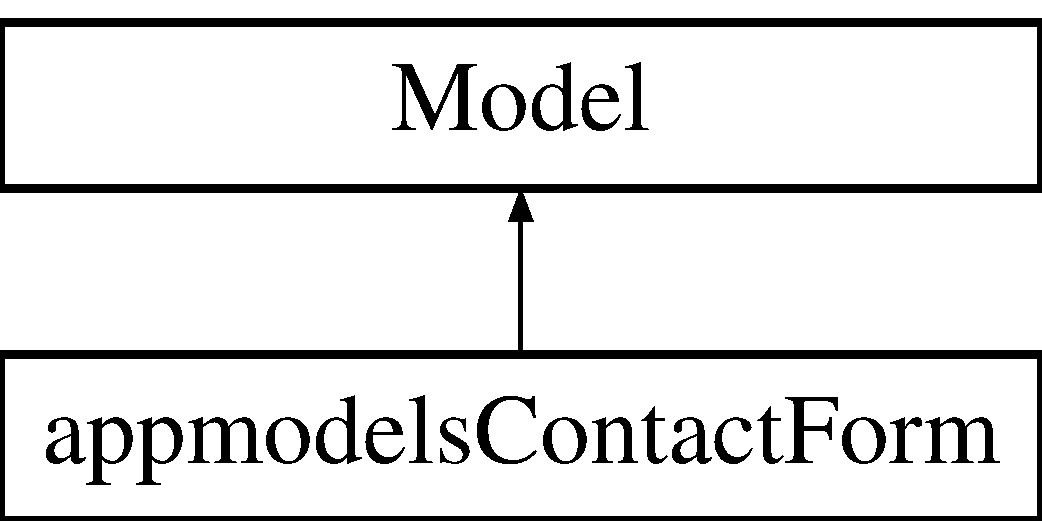
\includegraphics[height=2.000000cm]{classapp_1_1models_1_1ContactForm}
\end{center}
\end{figure}
\subsection*{Public Member Functions}
\begin{DoxyCompactItemize}
\item 
\hyperlink{classapp_1_1models_1_1ContactForm_a346c2c44cbe7a82c2e8f1de2f1958bb9}{rules} ()
\item 
\hyperlink{classapp_1_1models_1_1ContactForm_ad11e74305da95f8e2cd13d0eb15fe771}{attribute\+Labels} ()
\item 
\hyperlink{classapp_1_1models_1_1ContactForm_a42e6b6499a29df52c36ad4b2dfb2fe1a}{contact} (\$email)
\end{DoxyCompactItemize}
\subsection*{Public Attributes}
\begin{DoxyCompactItemize}
\end{DoxyCompactItemize}


\subsection{Detailed Description}
\hyperlink{classapp_1_1models_1_1ContactForm}{Contact\+Form} is the model behind the contact form. 

\subsection{Member Function Documentation}
\index{app\+::models\+::\+Contact\+Form@{app\+::models\+::\+Contact\+Form}!attribute\+Labels@{attribute\+Labels}}
\index{attribute\+Labels@{attribute\+Labels}!app\+::models\+::\+Contact\+Form@{app\+::models\+::\+Contact\+Form}}
\subsubsection[{\texorpdfstring{attribute\+Labels()}{attributeLabels()}}]{\setlength{\rightskip}{0pt plus 5cm}app\textbackslash{}models\textbackslash{}\+Contact\+Form\+::attribute\+Labels (
\begin{DoxyParamCaption}
{}
\end{DoxyParamCaption}
)}\hypertarget{classapp_1_1models_1_1ContactForm_ad11e74305da95f8e2cd13d0eb15fe771}{}\label{classapp_1_1models_1_1ContactForm_ad11e74305da95f8e2cd13d0eb15fe771}
\begin{DoxyReturn}{Returns}
array customized attribute labels 
\end{DoxyReturn}
\index{app\+::models\+::\+Contact\+Form@{app\+::models\+::\+Contact\+Form}!contact@{contact}}
\index{contact@{contact}!app\+::models\+::\+Contact\+Form@{app\+::models\+::\+Contact\+Form}}
\subsubsection[{\texorpdfstring{contact(\$email)}{contact($email)}}]{\setlength{\rightskip}{0pt plus 5cm}app\textbackslash{}models\textbackslash{}\+Contact\+Form\+::contact (
\begin{DoxyParamCaption}
\item[{}]{\$email}
\end{DoxyParamCaption}
)}\hypertarget{classapp_1_1models_1_1ContactForm_a42e6b6499a29df52c36ad4b2dfb2fe1a}{}\label{classapp_1_1models_1_1ContactForm_a42e6b6499a29df52c36ad4b2dfb2fe1a}
Sends an email to the specified email address using the information collected by this model. 
\begin{DoxyParams}[1]{Parameters}
string & {\em \$email} & the target email address \\
\hline
\end{DoxyParams}
\begin{DoxyReturn}{Returns}
boolean whether the model passes validation 
\end{DoxyReturn}
\index{app\+::models\+::\+Contact\+Form@{app\+::models\+::\+Contact\+Form}!rules@{rules}}
\index{rules@{rules}!app\+::models\+::\+Contact\+Form@{app\+::models\+::\+Contact\+Form}}
\subsubsection[{\texorpdfstring{rules()}{rules()}}]{\setlength{\rightskip}{0pt plus 5cm}app\textbackslash{}models\textbackslash{}\+Contact\+Form\+::rules (
\begin{DoxyParamCaption}
{}
\end{DoxyParamCaption}
)}\hypertarget{classapp_1_1models_1_1ContactForm_a346c2c44cbe7a82c2e8f1de2f1958bb9}{}\label{classapp_1_1models_1_1ContactForm_a346c2c44cbe7a82c2e8f1de2f1958bb9}
\begin{DoxyReturn}{Returns}
array the validation rules. 
\end{DoxyReturn}


The documentation for this class was generated from the following file\+:\begin{DoxyCompactItemize}
\item 
models/Contact\+Form.\+php\end{DoxyCompactItemize}

\hypertarget{classapp_1_1models_1_1Groupmembers}{}\section{app\textbackslash{}models\textbackslash{}Groupmembers Class Reference}
\label{classapp_1_1models_1_1Groupmembers}\index{app\textbackslash{}models\textbackslash{}\+Groupmembers@{app\textbackslash{}models\textbackslash{}\+Groupmembers}}
Inheritance diagram for app\textbackslash{}models\textbackslash{}Groupmembers\+:\begin{figure}[H]
\begin{center}
\leavevmode
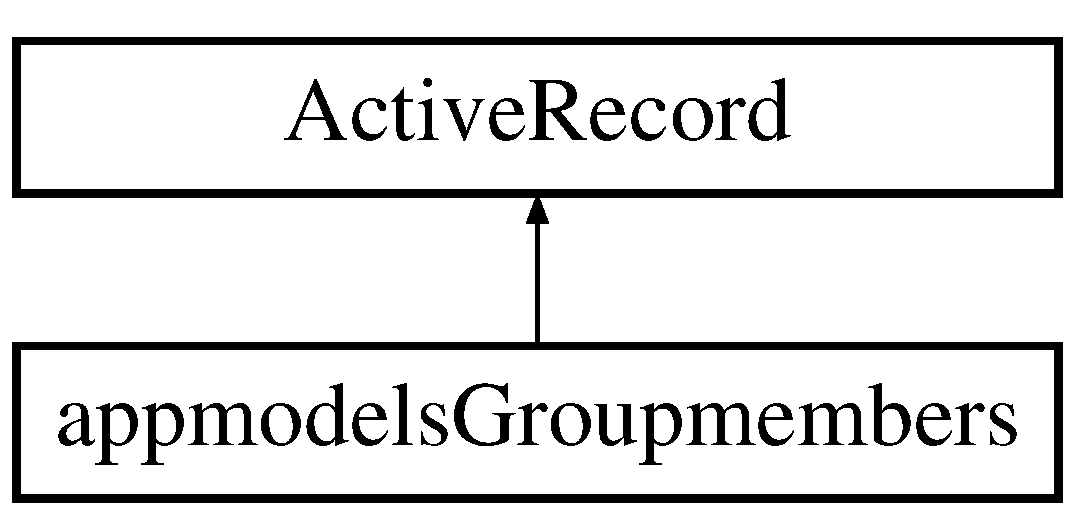
\includegraphics[height=2.000000cm]{classapp_1_1models_1_1Groupmembers}
\end{center}
\end{figure}
\subsection*{Public Member Functions}
\begin{DoxyCompactItemize}
\item 
\hyperlink{classapp_1_1models_1_1Groupmembers_a167dba82b81e6e1d88dc18680ad2cd6a}{rules} ()
\item 
\hyperlink{classapp_1_1models_1_1Groupmembers_ac5e6bcc73e98fd4693f17205d01c56b2}{attribute\+Labels} ()
\item 
\hyperlink{classapp_1_1models_1_1Groupmembers_a29bf461f6cdf4d2b4980108017819e87}{get\+Groupname0} ()
\end{DoxyCompactItemize}
\subsection*{Static Public Member Functions}
\begin{DoxyCompactItemize}
\item 
static \hyperlink{classapp_1_1models_1_1Groupmembers_a869e1a2959ec0776a2d08a47b821cb38}{table\+Name} ()
\end{DoxyCompactItemize}
\subsection*{Public Attributes}
\begin{DoxyCompactItemize}
\end{DoxyCompactItemize}


\subsection{Member Function Documentation}
\index{app\+::models\+::\+Groupmembers@{app\+::models\+::\+Groupmembers}!attribute\+Labels@{attribute\+Labels}}
\index{attribute\+Labels@{attribute\+Labels}!app\+::models\+::\+Groupmembers@{app\+::models\+::\+Groupmembers}}
\subsubsection[{\texorpdfstring{attribute\+Labels()}{attributeLabels()}}]{\setlength{\rightskip}{0pt plus 5cm}app\textbackslash{}models\textbackslash{}\+Groupmembers\+::attribute\+Labels (
\begin{DoxyParamCaption}
{}
\end{DoxyParamCaption}
)}\hypertarget{classapp_1_1models_1_1Groupmembers_ac5e6bcc73e98fd4693f17205d01c56b2}{}\label{classapp_1_1models_1_1Groupmembers_ac5e6bcc73e98fd4693f17205d01c56b2}
\index{app\+::models\+::\+Groupmembers@{app\+::models\+::\+Groupmembers}!get\+Groupname0@{get\+Groupname0}}
\index{get\+Groupname0@{get\+Groupname0}!app\+::models\+::\+Groupmembers@{app\+::models\+::\+Groupmembers}}
\subsubsection[{\texorpdfstring{get\+Groupname0()}{getGroupname0()}}]{\setlength{\rightskip}{0pt plus 5cm}app\textbackslash{}models\textbackslash{}\+Groupmembers\+::get\+Groupname0 (
\begin{DoxyParamCaption}
{}
\end{DoxyParamCaption}
)}\hypertarget{classapp_1_1models_1_1Groupmembers_a29bf461f6cdf4d2b4980108017819e87}{}\label{classapp_1_1models_1_1Groupmembers_a29bf461f6cdf4d2b4980108017819e87}
\begin{DoxyReturn}{Returns}

\end{DoxyReturn}
\index{app\+::models\+::\+Groupmembers@{app\+::models\+::\+Groupmembers}!rules@{rules}}
\index{rules@{rules}!app\+::models\+::\+Groupmembers@{app\+::models\+::\+Groupmembers}}
\subsubsection[{\texorpdfstring{rules()}{rules()}}]{\setlength{\rightskip}{0pt plus 5cm}app\textbackslash{}models\textbackslash{}\+Groupmembers\+::rules (
\begin{DoxyParamCaption}
{}
\end{DoxyParamCaption}
)}\hypertarget{classapp_1_1models_1_1Groupmembers_a167dba82b81e6e1d88dc18680ad2cd6a}{}\label{classapp_1_1models_1_1Groupmembers_a167dba82b81e6e1d88dc18680ad2cd6a}
\index{app\+::models\+::\+Groupmembers@{app\+::models\+::\+Groupmembers}!table\+Name@{table\+Name}}
\index{table\+Name@{table\+Name}!app\+::models\+::\+Groupmembers@{app\+::models\+::\+Groupmembers}}
\subsubsection[{\texorpdfstring{table\+Name()}{tableName()}}]{\setlength{\rightskip}{0pt plus 5cm}static app\textbackslash{}models\textbackslash{}\+Groupmembers\+::table\+Name (
\begin{DoxyParamCaption}
{}
\end{DoxyParamCaption}
)\hspace{0.3cm}{\ttfamily [static]}}\hypertarget{classapp_1_1models_1_1Groupmembers_a869e1a2959ec0776a2d08a47b821cb38}{}\label{classapp_1_1models_1_1Groupmembers_a869e1a2959ec0776a2d08a47b821cb38}


The documentation for this class was generated from the following file\+:\begin{DoxyCompactItemize}
\item 
models/Groupmembers.\+php\end{DoxyCompactItemize}

\hypertarget{classapp_1_1models_1_1Groups}{}\section{app\textbackslash{}models\textbackslash{}Groups Class Reference}
\label{classapp_1_1models_1_1Groups}\index{app\textbackslash{}models\textbackslash{}\+Groups@{app\textbackslash{}models\textbackslash{}\+Groups}}
Inheritance diagram for app\textbackslash{}models\textbackslash{}Groups\+:\begin{figure}[H]
\begin{center}
\leavevmode
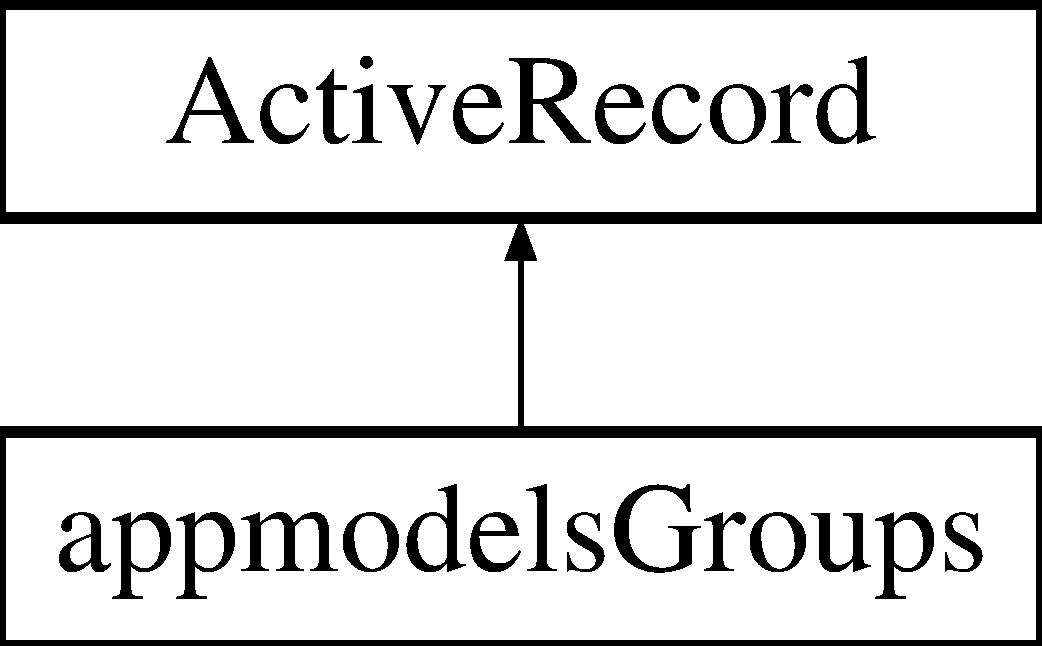
\includegraphics[height=2.000000cm]{classapp_1_1models_1_1Groups}
\end{center}
\end{figure}
\subsection*{Public Member Functions}
\begin{DoxyCompactItemize}
\item 
\hyperlink{classapp_1_1models_1_1Groups_aeabe4f44c6f2f23ce0afaa919f75c6e6}{rules} ()
\item 
\hyperlink{classapp_1_1models_1_1Groups_abdb0c0d59f1e0cb700e1e4e647d3e27c}{attribute\+Labels} ()
\item 
\hyperlink{classapp_1_1models_1_1Groups_a906bf4d4731c890146ca08317cad371a}{get\+Groupmembers} ()
\item 
\hyperlink{classapp_1_1models_1_1Groups_ae0e9983874d3b4f4cb29379c4e517f72}{group\+Exist} ()
\end{DoxyCompactItemize}
\subsection*{Static Public Member Functions}
\begin{DoxyCompactItemize}
\item 
static \hyperlink{classapp_1_1models_1_1Groups_af375acf39fc7b9e6cb0d1010959febc5}{table\+Name} ()
\item 
static \hyperlink{classapp_1_1models_1_1Groups_a13c20f87fc05f3010d793415707cc993}{find} ()
\end{DoxyCompactItemize}
\subsection*{Public Attributes}
\begin{DoxyCompactItemize}
\item 
\hyperlink{classapp_1_1models_1_1Groups_a856dc426eef888fa04f70e36a3d5b93d}{\$members}
\end{DoxyCompactItemize}


\subsection{Member Function Documentation}
\index{app\+::models\+::\+Groups@{app\+::models\+::\+Groups}!attribute\+Labels@{attribute\+Labels}}
\index{attribute\+Labels@{attribute\+Labels}!app\+::models\+::\+Groups@{app\+::models\+::\+Groups}}
\subsubsection[{\texorpdfstring{attribute\+Labels()}{attributeLabels()}}]{\setlength{\rightskip}{0pt plus 5cm}app\textbackslash{}models\textbackslash{}\+Groups\+::attribute\+Labels (
\begin{DoxyParamCaption}
{}
\end{DoxyParamCaption}
)}\hypertarget{classapp_1_1models_1_1Groups_abdb0c0d59f1e0cb700e1e4e647d3e27c}{}\label{classapp_1_1models_1_1Groups_abdb0c0d59f1e0cb700e1e4e647d3e27c}
\index{app\+::models\+::\+Groups@{app\+::models\+::\+Groups}!find@{find}}
\index{find@{find}!app\+::models\+::\+Groups@{app\+::models\+::\+Groups}}
\subsubsection[{\texorpdfstring{find()}{find()}}]{\setlength{\rightskip}{0pt plus 5cm}static app\textbackslash{}models\textbackslash{}\+Groups\+::find (
\begin{DoxyParamCaption}
{}
\end{DoxyParamCaption}
)\hspace{0.3cm}{\ttfamily [static]}}\hypertarget{classapp_1_1models_1_1Groups_a13c20f87fc05f3010d793415707cc993}{}\label{classapp_1_1models_1_1Groups_a13c20f87fc05f3010d793415707cc993}
\begin{DoxyReturn}{Returns}
\hyperlink{classapp_1_1models_1_1GroupsQuery}{Groups\+Query} the active query used by this AR class. 
\end{DoxyReturn}
\index{app\+::models\+::\+Groups@{app\+::models\+::\+Groups}!get\+Groupmembers@{get\+Groupmembers}}
\index{get\+Groupmembers@{get\+Groupmembers}!app\+::models\+::\+Groups@{app\+::models\+::\+Groups}}
\subsubsection[{\texorpdfstring{get\+Groupmembers()}{getGroupmembers()}}]{\setlength{\rightskip}{0pt plus 5cm}app\textbackslash{}models\textbackslash{}\+Groups\+::get\+Groupmembers (
\begin{DoxyParamCaption}
{}
\end{DoxyParamCaption}
)}\hypertarget{classapp_1_1models_1_1Groups_a906bf4d4731c890146ca08317cad371a}{}\label{classapp_1_1models_1_1Groups_a906bf4d4731c890146ca08317cad371a}
\begin{DoxyReturn}{Returns}

\end{DoxyReturn}
\index{app\+::models\+::\+Groups@{app\+::models\+::\+Groups}!group\+Exist@{group\+Exist}}
\index{group\+Exist@{group\+Exist}!app\+::models\+::\+Groups@{app\+::models\+::\+Groups}}
\subsubsection[{\texorpdfstring{group\+Exist()}{groupExist()}}]{\setlength{\rightskip}{0pt plus 5cm}app\textbackslash{}models\textbackslash{}\+Groups\+::group\+Exist (
\begin{DoxyParamCaption}
{}
\end{DoxyParamCaption}
)}\hypertarget{classapp_1_1models_1_1Groups_ae0e9983874d3b4f4cb29379c4e517f72}{}\label{classapp_1_1models_1_1Groups_ae0e9983874d3b4f4cb29379c4e517f72}
retrieve table groups \begin{DoxyReturn}{Returns}
true if found a match otherwise false 
\end{DoxyReturn}
\index{app\+::models\+::\+Groups@{app\+::models\+::\+Groups}!rules@{rules}}
\index{rules@{rules}!app\+::models\+::\+Groups@{app\+::models\+::\+Groups}}
\subsubsection[{\texorpdfstring{rules()}{rules()}}]{\setlength{\rightskip}{0pt plus 5cm}app\textbackslash{}models\textbackslash{}\+Groups\+::rules (
\begin{DoxyParamCaption}
{}
\end{DoxyParamCaption}
)}\hypertarget{classapp_1_1models_1_1Groups_aeabe4f44c6f2f23ce0afaa919f75c6e6}{}\label{classapp_1_1models_1_1Groups_aeabe4f44c6f2f23ce0afaa919f75c6e6}
\index{app\+::models\+::\+Groups@{app\+::models\+::\+Groups}!table\+Name@{table\+Name}}
\index{table\+Name@{table\+Name}!app\+::models\+::\+Groups@{app\+::models\+::\+Groups}}
\subsubsection[{\texorpdfstring{table\+Name()}{tableName()}}]{\setlength{\rightskip}{0pt plus 5cm}static app\textbackslash{}models\textbackslash{}\+Groups\+::table\+Name (
\begin{DoxyParamCaption}
{}
\end{DoxyParamCaption}
)\hspace{0.3cm}{\ttfamily [static]}}\hypertarget{classapp_1_1models_1_1Groups_af375acf39fc7b9e6cb0d1010959febc5}{}\label{classapp_1_1models_1_1Groups_af375acf39fc7b9e6cb0d1010959febc5}


\subsection{Member Data Documentation}
\index{app\+::models\+::\+Groups@{app\+::models\+::\+Groups}!\$members@{\$members}}
\index{\$members@{\$members}!app\+::models\+::\+Groups@{app\+::models\+::\+Groups}}
\subsubsection[{\texorpdfstring{\$members}{$members}}]{\setlength{\rightskip}{0pt plus 5cm}app\textbackslash{}models\textbackslash{}\+Groups\+::\$members}\hypertarget{classapp_1_1models_1_1Groups_a856dc426eef888fa04f70e36a3d5b93d}{}\label{classapp_1_1models_1_1Groups_a856dc426eef888fa04f70e36a3d5b93d}
a public variable. storing the group\+\_\+concat 

The documentation for this class was generated from the following file\+:\begin{DoxyCompactItemize}
\item 
models/Groups.\+php\end{DoxyCompactItemize}

\hypertarget{classapp_1_1models_1_1GroupsQuery}{}\section{app\textbackslash{}models\textbackslash{}Groups\+Query Class Reference}
\label{classapp_1_1models_1_1GroupsQuery}\index{app\textbackslash{}models\textbackslash{}\+Groups\+Query@{app\textbackslash{}models\textbackslash{}\+Groups\+Query}}
Inheritance diagram for app\textbackslash{}models\textbackslash{}Groups\+Query\+:\begin{figure}[H]
\begin{center}
\leavevmode
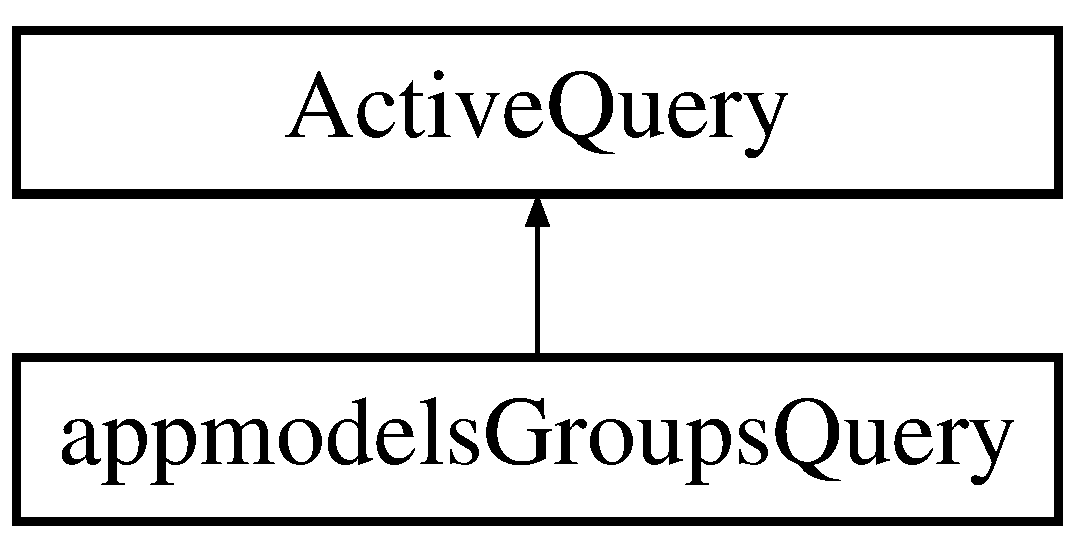
\includegraphics[height=2.000000cm]{classapp_1_1models_1_1GroupsQuery}
\end{center}
\end{figure}
\subsection*{Public Member Functions}
\begin{DoxyCompactItemize}
\item 
\hyperlink{classapp_1_1models_1_1GroupsQuery_a1d10ddb43497e1cf296db0fda4baa9cc}{all} (\$db=null)
\item 
\hyperlink{classapp_1_1models_1_1GroupsQuery_a50e817175f16850d7f7db59cffbb11b7}{one} (\$db=null)
\end{DoxyCompactItemize}


\subsection{Detailed Description}
This is the Active\+Query class for \mbox{[}\mbox{[}\hyperlink{classapp_1_1models_1_1Groups}{Groups}\mbox{]}\mbox{]}.

\begin{DoxySeeAlso}{See also}
\hyperlink{classapp_1_1models_1_1Groups}{Groups} 
\end{DoxySeeAlso}


\subsection{Member Function Documentation}
\index{app\+::models\+::\+Groups\+Query@{app\+::models\+::\+Groups\+Query}!all@{all}}
\index{all@{all}!app\+::models\+::\+Groups\+Query@{app\+::models\+::\+Groups\+Query}}
\subsubsection[{\texorpdfstring{all(\$db=null)}{all($db=null)}}]{\setlength{\rightskip}{0pt plus 5cm}app\textbackslash{}models\textbackslash{}\+Groups\+Query\+::all (
\begin{DoxyParamCaption}
\item[{}]{\$db = {\ttfamily null}}
\end{DoxyParamCaption}
)}\hypertarget{classapp_1_1models_1_1GroupsQuery_a1d10ddb43497e1cf296db0fda4baa9cc}{}\label{classapp_1_1models_1_1GroupsQuery_a1d10ddb43497e1cf296db0fda4baa9cc}
\begin{DoxyReturn}{Returns}
\hyperlink{classapp_1_1models_1_1Groups}{Groups}\mbox{[}\mbox{]}$\vert$array 
\end{DoxyReturn}
\index{app\+::models\+::\+Groups\+Query@{app\+::models\+::\+Groups\+Query}!one@{one}}
\index{one@{one}!app\+::models\+::\+Groups\+Query@{app\+::models\+::\+Groups\+Query}}
\subsubsection[{\texorpdfstring{one(\$db=null)}{one($db=null)}}]{\setlength{\rightskip}{0pt plus 5cm}app\textbackslash{}models\textbackslash{}\+Groups\+Query\+::one (
\begin{DoxyParamCaption}
\item[{}]{\$db = {\ttfamily null}}
\end{DoxyParamCaption}
)}\hypertarget{classapp_1_1models_1_1GroupsQuery_a50e817175f16850d7f7db59cffbb11b7}{}\label{classapp_1_1models_1_1GroupsQuery_a50e817175f16850d7f7db59cffbb11b7}
\begin{DoxyReturn}{Returns}
Groups$\vert$array$\vert$null 
\end{DoxyReturn}


The documentation for this class was generated from the following file\+:\begin{DoxyCompactItemize}
\item 
models/Groups\+Query.\+php\end{DoxyCompactItemize}

\hypertarget{classapp_1_1models_1_1LoginForm}{}\section{app\textbackslash{}models\textbackslash{}Login\+Form Class Reference}
\label{classapp_1_1models_1_1LoginForm}\index{app\textbackslash{}models\textbackslash{}\+Login\+Form@{app\textbackslash{}models\textbackslash{}\+Login\+Form}}
Inheritance diagram for app\textbackslash{}models\textbackslash{}Login\+Form\+:\begin{figure}[H]
\begin{center}
\leavevmode
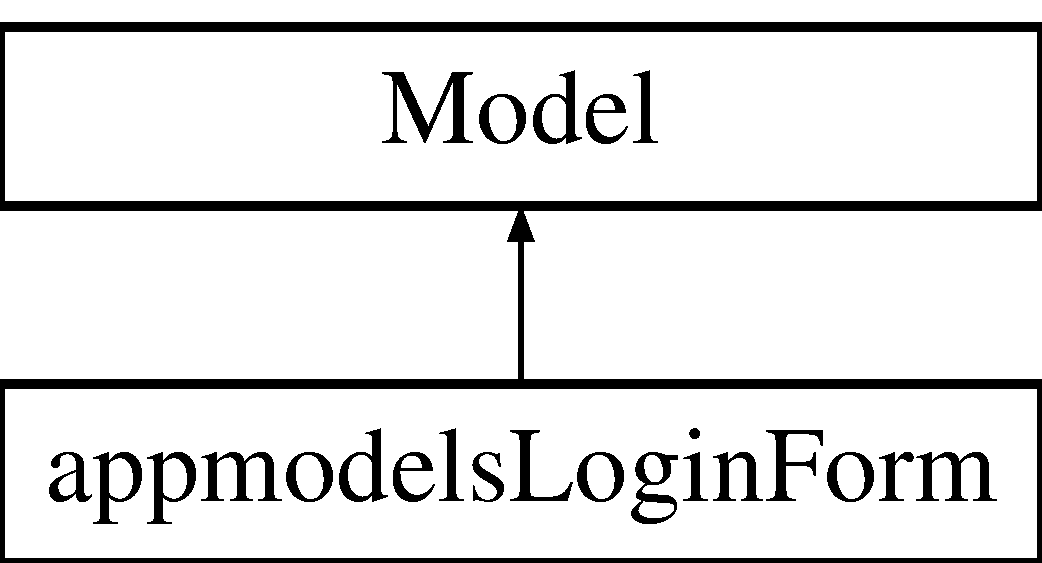
\includegraphics[height=2.000000cm]{classapp_1_1models_1_1LoginForm}
\end{center}
\end{figure}
\subsection*{Public Member Functions}
\begin{DoxyCompactItemize}
\item 
\hyperlink{classapp_1_1models_1_1LoginForm_ae8fce695061e13aea1f01114a49f2ab5}{rules} ()
\item 
\hyperlink{classapp_1_1models_1_1LoginForm_ab18ca60438364b0e4781e0d54855c641}{validate\+Password} (\$attribute, \$params)
\item 
\hyperlink{classapp_1_1models_1_1LoginForm_a934b2fb03be75b656cc23fd59f6619f4}{login} ()
\item 
\hyperlink{classapp_1_1models_1_1LoginForm_aff4dcbbf9b5a3e1f433cb4f88343d54a}{get\+User} ()
\end{DoxyCompactItemize}
\subsection*{Public Attributes}
\begin{DoxyCompactItemize}
\end{DoxyCompactItemize}


\subsection{Detailed Description}
\hyperlink{classapp_1_1models_1_1LoginForm}{Login\+Form} is the model behind the login form. 

\subsection{Member Function Documentation}
\index{app\+::models\+::\+Login\+Form@{app\+::models\+::\+Login\+Form}!get\+User@{get\+User}}
\index{get\+User@{get\+User}!app\+::models\+::\+Login\+Form@{app\+::models\+::\+Login\+Form}}
\subsubsection[{\texorpdfstring{get\+User()}{getUser()}}]{\setlength{\rightskip}{0pt plus 5cm}app\textbackslash{}models\textbackslash{}\+Login\+Form\+::get\+User (
\begin{DoxyParamCaption}
{}
\end{DoxyParamCaption}
)}\hypertarget{classapp_1_1models_1_1LoginForm_aff4dcbbf9b5a3e1f433cb4f88343d54a}{}\label{classapp_1_1models_1_1LoginForm_aff4dcbbf9b5a3e1f433cb4f88343d54a}
Finds user by \mbox{[}\mbox{[}username\mbox{]}\mbox{]}

\begin{DoxyReturn}{Returns}
User$\vert$null 
\end{DoxyReturn}
\index{app\+::models\+::\+Login\+Form@{app\+::models\+::\+Login\+Form}!login@{login}}
\index{login@{login}!app\+::models\+::\+Login\+Form@{app\+::models\+::\+Login\+Form}}
\subsubsection[{\texorpdfstring{login()}{login()}}]{\setlength{\rightskip}{0pt plus 5cm}app\textbackslash{}models\textbackslash{}\+Login\+Form\+::login (
\begin{DoxyParamCaption}
{}
\end{DoxyParamCaption}
)}\hypertarget{classapp_1_1models_1_1LoginForm_a934b2fb03be75b656cc23fd59f6619f4}{}\label{classapp_1_1models_1_1LoginForm_a934b2fb03be75b656cc23fd59f6619f4}
Logs in a user using the provided username and password. \begin{DoxyReturn}{Returns}
boolean whether the user is logged in successfully 
\end{DoxyReturn}
\index{app\+::models\+::\+Login\+Form@{app\+::models\+::\+Login\+Form}!rules@{rules}}
\index{rules@{rules}!app\+::models\+::\+Login\+Form@{app\+::models\+::\+Login\+Form}}
\subsubsection[{\texorpdfstring{rules()}{rules()}}]{\setlength{\rightskip}{0pt plus 5cm}app\textbackslash{}models\textbackslash{}\+Login\+Form\+::rules (
\begin{DoxyParamCaption}
{}
\end{DoxyParamCaption}
)}\hypertarget{classapp_1_1models_1_1LoginForm_ae8fce695061e13aea1f01114a49f2ab5}{}\label{classapp_1_1models_1_1LoginForm_ae8fce695061e13aea1f01114a49f2ab5}
\begin{DoxyReturn}{Returns}
array the validation rules. 
\end{DoxyReturn}
\index{app\+::models\+::\+Login\+Form@{app\+::models\+::\+Login\+Form}!validate\+Password@{validate\+Password}}
\index{validate\+Password@{validate\+Password}!app\+::models\+::\+Login\+Form@{app\+::models\+::\+Login\+Form}}
\subsubsection[{\texorpdfstring{validate\+Password(\$attribute, \$params)}{validatePassword($attribute, $params)}}]{\setlength{\rightskip}{0pt plus 5cm}app\textbackslash{}models\textbackslash{}\+Login\+Form\+::validate\+Password (
\begin{DoxyParamCaption}
\item[{}]{\$attribute, }
\item[{}]{\$params}
\end{DoxyParamCaption}
)}\hypertarget{classapp_1_1models_1_1LoginForm_ab18ca60438364b0e4781e0d54855c641}{}\label{classapp_1_1models_1_1LoginForm_ab18ca60438364b0e4781e0d54855c641}
Validates the password. This method serves as the inline validation for password.


\begin{DoxyParams}[1]{Parameters}
string & {\em \$attribute} & the attribute currently being validated \\
\hline
array & {\em \$params} & the additional name-\/value pairs given in the rule \\
\hline
\end{DoxyParams}


The documentation for this class was generated from the following file\+:\begin{DoxyCompactItemize}
\item 
models/Login\+Form.\+php\end{DoxyCompactItemize}

\hypertarget{classapp_1_1models_1_1ProfileForm}{}\section{app\textbackslash{}models\textbackslash{}Profile\+Form Class Reference}
\label{classapp_1_1models_1_1ProfileForm}\index{app\textbackslash{}models\textbackslash{}\+Profile\+Form@{app\textbackslash{}models\textbackslash{}\+Profile\+Form}}
Inheritance diagram for app\textbackslash{}models\textbackslash{}Profile\+Form\+:\begin{figure}[H]
\begin{center}
\leavevmode
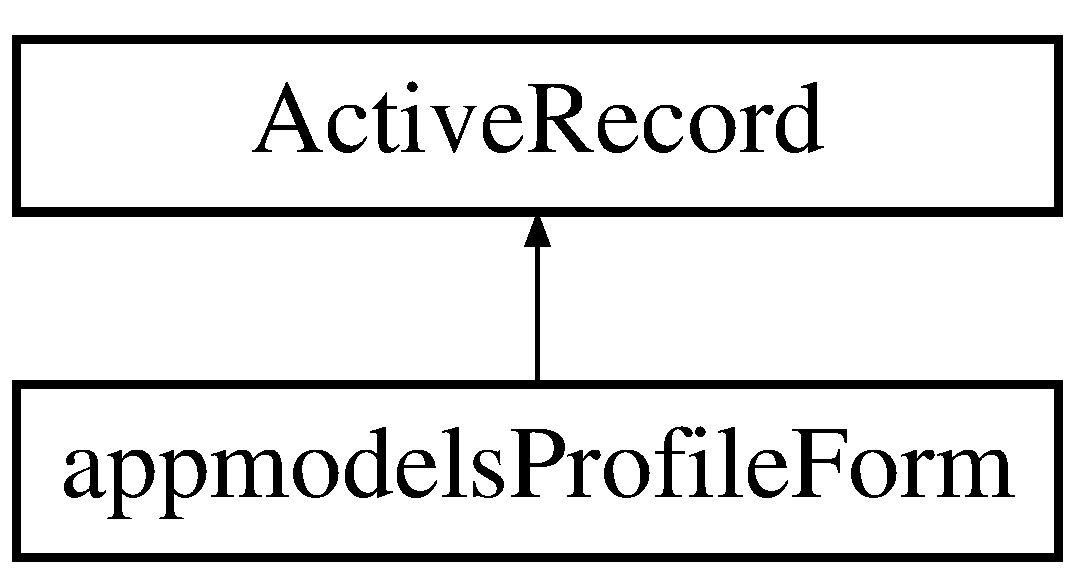
\includegraphics[height=2.000000cm]{classapp_1_1models_1_1ProfileForm}
\end{center}
\end{figure}
\subsection*{Public Member Functions}
\begin{DoxyCompactItemize}
\item 
\hyperlink{classapp_1_1models_1_1ProfileForm_ae6a8f3dd460d3ff4377f62f234be6ee9}{rules} ()
\item 
\hyperlink{classapp_1_1models_1_1ProfileForm_a685a2817afeedb9d103743959ad975ca}{attribute\+Labels} ()
\item 
\hyperlink{classapp_1_1models_1_1ProfileForm_ae7b0dbbff0b01febacd6025337f72dfc}{initialize} ()
\item 
\hyperlink{classapp_1_1models_1_1ProfileForm_a781f53269dc3f3974932497284d10a7e}{test\+\_\+initialize} ()
\item 
\hyperlink{classapp_1_1models_1_1ProfileForm_a63d6177515a6a73f568ca0a9360ab1fb}{add\+User\+Profile} (\$user, \$signupfrom)
\end{DoxyCompactItemize}
\subsection*{Static Public Member Functions}
\begin{DoxyCompactItemize}
\item 
static \hyperlink{classapp_1_1models_1_1ProfileForm_aeef44bfb431e7410e7c57000e6790032}{table\+Name} ()
\end{DoxyCompactItemize}


\subsection{Member Function Documentation}
\index{app\+::models\+::\+Profile\+Form@{app\+::models\+::\+Profile\+Form}!add\+User\+Profile@{add\+User\+Profile}}
\index{add\+User\+Profile@{add\+User\+Profile}!app\+::models\+::\+Profile\+Form@{app\+::models\+::\+Profile\+Form}}
\subsubsection[{\texorpdfstring{add\+User\+Profile(\$user, \$signupfrom)}{addUserProfile($user, $signupfrom)}}]{\setlength{\rightskip}{0pt plus 5cm}app\textbackslash{}models\textbackslash{}\+Profile\+Form\+::add\+User\+Profile (
\begin{DoxyParamCaption}
\item[{}]{\$user, }
\item[{}]{\$signupfrom}
\end{DoxyParamCaption}
)}\hypertarget{classapp_1_1models_1_1ProfileForm_a63d6177515a6a73f568ca0a9360ab1fb}{}\label{classapp_1_1models_1_1ProfileForm_a63d6177515a6a73f568ca0a9360ab1fb}
Update Profile if existing, Add if the record is new


\begin{DoxyParams}{Parameters}
{\em \$user} & Object \hyperlink{classapp_1_1models_1_1User}{User} \\
\hline
{\em \$signupform} & Object \hyperlink{classapp_1_1models_1_1SignupForm}{Signup\+Form} \\
\hline
\end{DoxyParams}
\begin{DoxyReturn}{Returns}
boolean if password provided is valid for current user 
\end{DoxyReturn}
\index{app\+::models\+::\+Profile\+Form@{app\+::models\+::\+Profile\+Form}!attribute\+Labels@{attribute\+Labels}}
\index{attribute\+Labels@{attribute\+Labels}!app\+::models\+::\+Profile\+Form@{app\+::models\+::\+Profile\+Form}}
\subsubsection[{\texorpdfstring{attribute\+Labels()}{attributeLabels()}}]{\setlength{\rightskip}{0pt plus 5cm}app\textbackslash{}models\textbackslash{}\+Profile\+Form\+::attribute\+Labels (
\begin{DoxyParamCaption}
{}
\end{DoxyParamCaption}
)}\hypertarget{classapp_1_1models_1_1ProfileForm_a685a2817afeedb9d103743959ad975ca}{}\label{classapp_1_1models_1_1ProfileForm_a685a2817afeedb9d103743959ad975ca}
\index{app\+::models\+::\+Profile\+Form@{app\+::models\+::\+Profile\+Form}!initialize@{initialize}}
\index{initialize@{initialize}!app\+::models\+::\+Profile\+Form@{app\+::models\+::\+Profile\+Form}}
\subsubsection[{\texorpdfstring{initialize()}{initialize()}}]{\setlength{\rightskip}{0pt plus 5cm}app\textbackslash{}models\textbackslash{}\+Profile\+Form\+::initialize (
\begin{DoxyParamCaption}
{}
\end{DoxyParamCaption}
)}\hypertarget{classapp_1_1models_1_1ProfileForm_ae7b0dbbff0b01febacd6025337f72dfc}{}\label{classapp_1_1models_1_1ProfileForm_ae7b0dbbff0b01febacd6025337f72dfc}
initializing the object (test1)

\begin{DoxyReturn}{Returns}
None 
\end{DoxyReturn}
\index{app\+::models\+::\+Profile\+Form@{app\+::models\+::\+Profile\+Form}!rules@{rules}}
\index{rules@{rules}!app\+::models\+::\+Profile\+Form@{app\+::models\+::\+Profile\+Form}}
\subsubsection[{\texorpdfstring{rules()}{rules()}}]{\setlength{\rightskip}{0pt plus 5cm}app\textbackslash{}models\textbackslash{}\+Profile\+Form\+::rules (
\begin{DoxyParamCaption}
{}
\end{DoxyParamCaption}
)}\hypertarget{classapp_1_1models_1_1ProfileForm_ae6a8f3dd460d3ff4377f62f234be6ee9}{}\label{classapp_1_1models_1_1ProfileForm_ae6a8f3dd460d3ff4377f62f234be6ee9}
\index{app\+::models\+::\+Profile\+Form@{app\+::models\+::\+Profile\+Form}!table\+Name@{table\+Name}}
\index{table\+Name@{table\+Name}!app\+::models\+::\+Profile\+Form@{app\+::models\+::\+Profile\+Form}}
\subsubsection[{\texorpdfstring{table\+Name()}{tableName()}}]{\setlength{\rightskip}{0pt plus 5cm}static app\textbackslash{}models\textbackslash{}\+Profile\+Form\+::table\+Name (
\begin{DoxyParamCaption}
{}
\end{DoxyParamCaption}
)\hspace{0.3cm}{\ttfamily [static]}}\hypertarget{classapp_1_1models_1_1ProfileForm_aeef44bfb431e7410e7c57000e6790032}{}\label{classapp_1_1models_1_1ProfileForm_aeef44bfb431e7410e7c57000e6790032}
\index{app\+::models\+::\+Profile\+Form@{app\+::models\+::\+Profile\+Form}!test\+\_\+initialize@{test\+\_\+initialize}}
\index{test\+\_\+initialize@{test\+\_\+initialize}!app\+::models\+::\+Profile\+Form@{app\+::models\+::\+Profile\+Form}}
\subsubsection[{\texorpdfstring{test\+\_\+initialize()}{test_initialize()}}]{\setlength{\rightskip}{0pt plus 5cm}app\textbackslash{}models\textbackslash{}\+Profile\+Form\+::test\+\_\+initialize (
\begin{DoxyParamCaption}
{}
\end{DoxyParamCaption}
)}\hypertarget{classapp_1_1models_1_1ProfileForm_a781f53269dc3f3974932497284d10a7e}{}\label{classapp_1_1models_1_1ProfileForm_a781f53269dc3f3974932497284d10a7e}
initializing the object (test2)

\begin{DoxyReturn}{Returns}
None 
\end{DoxyReturn}


The documentation for this class was generated from the following file\+:\begin{DoxyCompactItemize}
\item 
models/Profile\+Form.\+php\end{DoxyCompactItemize}

\hypertarget{classapp_1_1models_1_1SignupForm}{}\section{app\textbackslash{}models\textbackslash{}Signup\+Form Class Reference}
\label{classapp_1_1models_1_1SignupForm}\index{app\textbackslash{}models\textbackslash{}\+Signup\+Form@{app\textbackslash{}models\textbackslash{}\+Signup\+Form}}
Inheritance diagram for app\textbackslash{}models\textbackslash{}Signup\+Form\+:\begin{figure}[H]
\begin{center}
\leavevmode
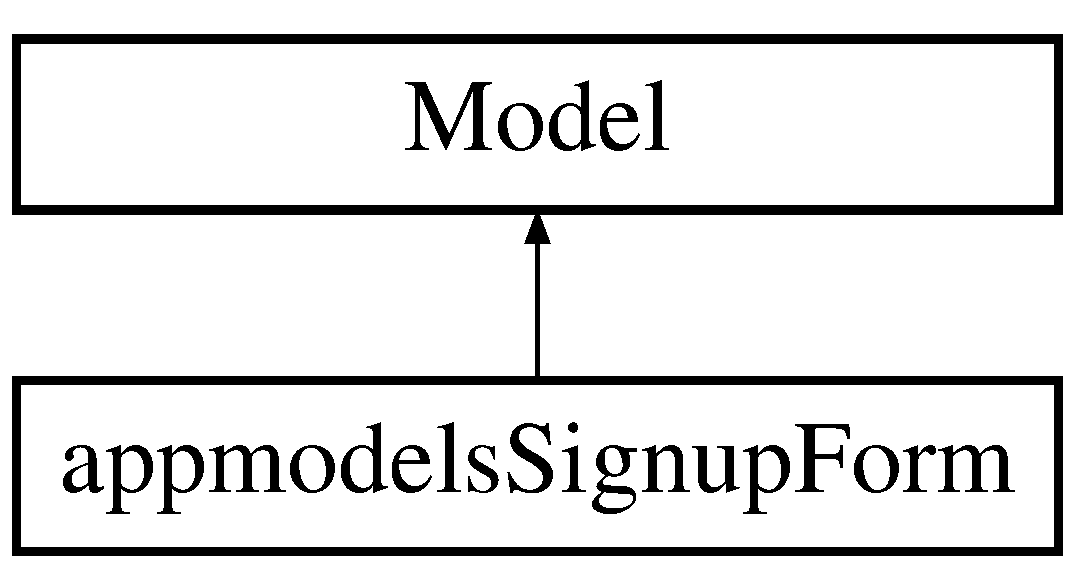
\includegraphics[height=2.000000cm]{classapp_1_1models_1_1SignupForm}
\end{center}
\end{figure}
\subsection*{Public Member Functions}
\begin{DoxyCompactItemize}
\item 
\hyperlink{classapp_1_1models_1_1SignupForm_afeadbfcda7896631b6330be330f6d596}{release\+Error\+Model} ()
\item 
\hyperlink{classapp_1_1models_1_1SignupForm_ad9bb86cb0b4146eafa0eb40bb65740bd}{user\+Exist} (\$attribute, \$params)
\end{DoxyCompactItemize}
\subsection*{Public Attributes}
\begin{DoxyCompactItemize}
\end{DoxyCompactItemize}


\subsection{Member Function Documentation}
\index{app\+::models\+::\+Signup\+Form@{app\+::models\+::\+Signup\+Form}!release\+Error\+Model@{release\+Error\+Model}}
\index{release\+Error\+Model@{release\+Error\+Model}!app\+::models\+::\+Signup\+Form@{app\+::models\+::\+Signup\+Form}}
\subsubsection[{\texorpdfstring{release\+Error\+Model()}{releaseErrorModel()}}]{\setlength{\rightskip}{0pt plus 5cm}app\textbackslash{}models\textbackslash{}\+Signup\+Form\+::release\+Error\+Model (
\begin{DoxyParamCaption}
{}
\end{DoxyParamCaption}
)}\hypertarget{classapp_1_1models_1_1SignupForm_afeadbfcda7896631b6330be330f6d596}{}\label{classapp_1_1models_1_1SignupForm_afeadbfcda7896631b6330be330f6d596}
modify the value of the variables of current object return \$this \index{app\+::models\+::\+Signup\+Form@{app\+::models\+::\+Signup\+Form}!user\+Exist@{user\+Exist}}
\index{user\+Exist@{user\+Exist}!app\+::models\+::\+Signup\+Form@{app\+::models\+::\+Signup\+Form}}
\subsubsection[{\texorpdfstring{user\+Exist(\$attribute, \$params)}{userExist($attribute, $params)}}]{\setlength{\rightskip}{0pt plus 5cm}app\textbackslash{}models\textbackslash{}\+Signup\+Form\+::user\+Exist (
\begin{DoxyParamCaption}
\item[{}]{\$attribute, }
\item[{}]{\$params}
\end{DoxyParamCaption}
)}\hypertarget{classapp_1_1models_1_1SignupForm_ad9bb86cb0b4146eafa0eb40bb65740bd}{}\label{classapp_1_1models_1_1SignupForm_ad9bb86cb0b4146eafa0eb40bb65740bd}
Add error to Signup Form \& change password to empty 
\begin{DoxyParams}[1]{Parameters}
type & {\em \$attribute} & \\
\hline
type & {\em \$params} & \\
\hline
\end{DoxyParams}


The documentation for this class was generated from the following file\+:\begin{DoxyCompactItemize}
\item 
models/Signup\+Form.\+php\end{DoxyCompactItemize}

\hypertarget{classapp_1_1controllers_1_1SiteController}{}\section{app\textbackslash{}controllers\textbackslash{}Site\+Controller Class Reference}
\label{classapp_1_1controllers_1_1SiteController}\index{app\textbackslash{}controllers\textbackslash{}\+Site\+Controller@{app\textbackslash{}controllers\textbackslash{}\+Site\+Controller}}
Inheritance diagram for app\textbackslash{}controllers\textbackslash{}Site\+Controller\+:\begin{figure}[H]
\begin{center}
\leavevmode
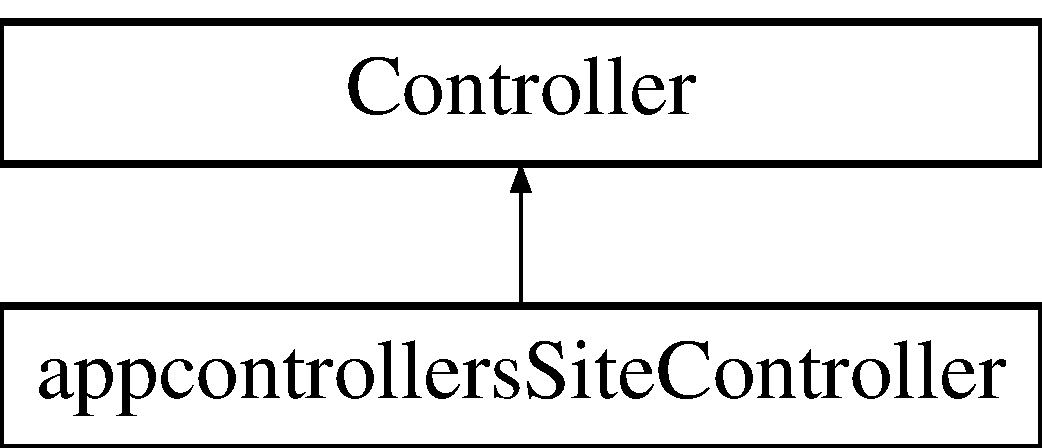
\includegraphics[height=2.000000cm]{classapp_1_1controllers_1_1SiteController}
\end{center}
\end{figure}
\subsection*{Public Member Functions}
\begin{DoxyCompactItemize}
\item 
\hyperlink{classapp_1_1controllers_1_1SiteController_a1c407c5da3459795a0c27d80eaaab5cb}{action\+Signup} ()
\item 
\hyperlink{classapp_1_1controllers_1_1SiteController_a2444906d12a76df58f9e75acf2c6f37f}{action\+Signup\+Success} (\$model)
\item 
\hyperlink{classapp_1_1controllers_1_1SiteController_a63074c19d6f5bd216a72955b0224c042}{action\+Creategroup} ()
\item 
\hyperlink{classapp_1_1controllers_1_1SiteController_a054da8f149f0a2226f509956fad6c3d4}{action\+View\+Group} ()
\item 
\hyperlink{classapp_1_1controllers_1_1SiteController_ace13521ef9b29a1d9b25c3cfb377c357}{action\+User\+Action} ()
\item 
\hyperlink{classapp_1_1controllers_1_1SiteController_a996f13d312c12ddda17298aa0e79a17f}{action\+Search\+Group} ()
\item 
\hyperlink{classapp_1_1controllers_1_1SiteController_add33feeb1946dca691b17c3929e6ad57}{action\+Profile} ()
\item 
\hyperlink{classapp_1_1controllers_1_1SiteController_aadfebaf8b8da2faf40149c0d98d93eb0}{action\+Say} (\$message)
\item 
\hyperlink{classapp_1_1controllers_1_1SiteController_abdee6c5abd4a3b8e633eef175942e46e}{action\+Index} ()
\item 
\hyperlink{classapp_1_1controllers_1_1SiteController_a8ad883ecfb857fc94c385f914ad06c5b}{action\+Login} ()
\end{DoxyCompactItemize}


\subsection{Member Function Documentation}
\index{app\+::controllers\+::\+Site\+Controller@{app\+::controllers\+::\+Site\+Controller}!action\+Creategroup@{action\+Creategroup}}
\index{action\+Creategroup@{action\+Creategroup}!app\+::controllers\+::\+Site\+Controller@{app\+::controllers\+::\+Site\+Controller}}
\subsubsection[{\texorpdfstring{action\+Creategroup()}{actionCreategroup()}}]{\setlength{\rightskip}{0pt plus 5cm}app\textbackslash{}controllers\textbackslash{}\+Site\+Controller\+::action\+Creategroup (
\begin{DoxyParamCaption}
{}
\end{DoxyParamCaption}
)}\hypertarget{classapp_1_1controllers_1_1SiteController_a63074c19d6f5bd216a72955b0224c042}{}\label{classapp_1_1controllers_1_1SiteController_a63074c19d6f5bd216a72955b0224c042}
render Creategroup.\+php with \$model = new Groups();

\begin{DoxyReturn}{Returns}
\$this-\/$>$render(\textquotesingle{}signup\textquotesingle{}, \mbox{[}\textquotesingle{}model\textquotesingle{} =$>$ \$model\mbox{]}) 
\end{DoxyReturn}
\index{app\+::controllers\+::\+Site\+Controller@{app\+::controllers\+::\+Site\+Controller}!action\+Index@{action\+Index}}
\index{action\+Index@{action\+Index}!app\+::controllers\+::\+Site\+Controller@{app\+::controllers\+::\+Site\+Controller}}
\subsubsection[{\texorpdfstring{action\+Index()}{actionIndex()}}]{\setlength{\rightskip}{0pt plus 5cm}app\textbackslash{}controllers\textbackslash{}\+Site\+Controller\+::action\+Index (
\begin{DoxyParamCaption}
{}
\end{DoxyParamCaption}
)}\hypertarget{classapp_1_1controllers_1_1SiteController_abdee6c5abd4a3b8e633eef175942e46e}{}\label{classapp_1_1controllers_1_1SiteController_abdee6c5abd4a3b8e633eef175942e46e}
render Index.\+php or view-\/group.\+php

\begin{DoxyReturn}{Returns}
\$this-\/$>$render(\textquotesingle{}index\textquotesingle{}) if not logged in otherwise \$this-\/$>$\hyperlink{classapp_1_1controllers_1_1SiteController_a054da8f149f0a2226f509956fad6c3d4}{action\+View\+Group()} 
\end{DoxyReturn}
\index{app\+::controllers\+::\+Site\+Controller@{app\+::controllers\+::\+Site\+Controller}!action\+Login@{action\+Login}}
\index{action\+Login@{action\+Login}!app\+::controllers\+::\+Site\+Controller@{app\+::controllers\+::\+Site\+Controller}}
\subsubsection[{\texorpdfstring{action\+Login()}{actionLogin()}}]{\setlength{\rightskip}{0pt plus 5cm}app\textbackslash{}controllers\textbackslash{}\+Site\+Controller\+::action\+Login (
\begin{DoxyParamCaption}
{}
\end{DoxyParamCaption}
)}\hypertarget{classapp_1_1controllers_1_1SiteController_a8ad883ecfb857fc94c385f914ad06c5b}{}\label{classapp_1_1controllers_1_1SiteController_a8ad883ecfb857fc94c385f914ad06c5b}
render login.\+php or view-\/group.\+php with Param \$model = Login\+Form

\begin{DoxyReturn}{Returns}
\$this-\/$>$render(\textquotesingle{}login\textquotesingle{}, \mbox{[}\textquotesingle{}model\textquotesingle{} =$>$ \$model,\mbox{]}) 
\end{DoxyReturn}
\index{app\+::controllers\+::\+Site\+Controller@{app\+::controllers\+::\+Site\+Controller}!action\+Profile@{action\+Profile}}
\index{action\+Profile@{action\+Profile}!app\+::controllers\+::\+Site\+Controller@{app\+::controllers\+::\+Site\+Controller}}
\subsubsection[{\texorpdfstring{action\+Profile()}{actionProfile()}}]{\setlength{\rightskip}{0pt plus 5cm}app\textbackslash{}controllers\textbackslash{}\+Site\+Controller\+::action\+Profile (
\begin{DoxyParamCaption}
{}
\end{DoxyParamCaption}
)}\hypertarget{classapp_1_1controllers_1_1SiteController_add33feeb1946dca691b17c3929e6ad57}{}\label{classapp_1_1controllers_1_1SiteController_add33feeb1946dca691b17c3929e6ad57}
render Profile.\+php with \$model as Profile\+Form if found profile; render Say.\+php with array.\+key = title, message

\begin{DoxyReturn}{Returns}
\$this-\/$>$render(\textquotesingle{}Join\+Group\textquotesingle{}, array) or \$this-\/$>$render(\textquotesingle{}Say\textquotesingle{}, array) 
\end{DoxyReturn}
\index{app\+::controllers\+::\+Site\+Controller@{app\+::controllers\+::\+Site\+Controller}!action\+Say@{action\+Say}}
\index{action\+Say@{action\+Say}!app\+::controllers\+::\+Site\+Controller@{app\+::controllers\+::\+Site\+Controller}}
\subsubsection[{\texorpdfstring{action\+Say(\$message)}{actionSay($message)}}]{\setlength{\rightskip}{0pt plus 5cm}app\textbackslash{}controllers\textbackslash{}\+Site\+Controller\+::action\+Say (
\begin{DoxyParamCaption}
\item[{}]{\$message}
\end{DoxyParamCaption}
)}\hypertarget{classapp_1_1controllers_1_1SiteController_aadfebaf8b8da2faf40149c0d98d93eb0}{}\label{classapp_1_1controllers_1_1SiteController_aadfebaf8b8da2faf40149c0d98d93eb0}
render Say.\+php with array.\+key = message

\begin{DoxyReturn}{Returns}
\$this-\/$>$render(\textquotesingle{}say\textquotesingle{}, array) 
\end{DoxyReturn}
\index{app\+::controllers\+::\+Site\+Controller@{app\+::controllers\+::\+Site\+Controller}!action\+Search\+Group@{action\+Search\+Group}}
\index{action\+Search\+Group@{action\+Search\+Group}!app\+::controllers\+::\+Site\+Controller@{app\+::controllers\+::\+Site\+Controller}}
\subsubsection[{\texorpdfstring{action\+Search\+Group()}{actionSearchGroup()}}]{\setlength{\rightskip}{0pt plus 5cm}app\textbackslash{}controllers\textbackslash{}\+Site\+Controller\+::action\+Search\+Group (
\begin{DoxyParamCaption}
{}
\end{DoxyParamCaption}
)}\hypertarget{classapp_1_1controllers_1_1SiteController_a996f13d312c12ddda17298aa0e79a17f}{}\label{classapp_1_1controllers_1_1SiteController_a996f13d312c12ddda17298aa0e79a17f}
render Join\+Group.\+php with array.\+key = Groups, keywords

\begin{DoxyReturn}{Returns}
\$this-\/$>$render(\textquotesingle{}Join\+Group\textquotesingle{}, array) 
\end{DoxyReturn}
\index{app\+::controllers\+::\+Site\+Controller@{app\+::controllers\+::\+Site\+Controller}!action\+Signup@{action\+Signup}}
\index{action\+Signup@{action\+Signup}!app\+::controllers\+::\+Site\+Controller@{app\+::controllers\+::\+Site\+Controller}}
\subsubsection[{\texorpdfstring{action\+Signup()}{actionSignup()}}]{\setlength{\rightskip}{0pt plus 5cm}app\textbackslash{}controllers\textbackslash{}\+Site\+Controller\+::action\+Signup (
\begin{DoxyParamCaption}
{}
\end{DoxyParamCaption}
)}\hypertarget{classapp_1_1controllers_1_1SiteController_a1c407c5da3459795a0c27d80eaaab5cb}{}\label{classapp_1_1controllers_1_1SiteController_a1c407c5da3459795a0c27d80eaaab5cb}
render Signup.\+php with \$model = new Signup\+Form();

\begin{DoxyReturn}{Returns}
\$this-\/$>$render(\textquotesingle{}signup\textquotesingle{}, \mbox{[}\textquotesingle{}model\textquotesingle{} =$>$ \$model\mbox{]}) 
\end{DoxyReturn}
$<$ activate the rule \index{app\+::controllers\+::\+Site\+Controller@{app\+::controllers\+::\+Site\+Controller}!action\+Signup\+Success@{action\+Signup\+Success}}
\index{action\+Signup\+Success@{action\+Signup\+Success}!app\+::controllers\+::\+Site\+Controller@{app\+::controllers\+::\+Site\+Controller}}
\subsubsection[{\texorpdfstring{action\+Signup\+Success(\$model)}{actionSignupSuccess($model)}}]{\setlength{\rightskip}{0pt plus 5cm}app\textbackslash{}controllers\textbackslash{}\+Site\+Controller\+::action\+Signup\+Success (
\begin{DoxyParamCaption}
\item[{}]{\$model}
\end{DoxyParamCaption}
)}\hypertarget{classapp_1_1controllers_1_1SiteController_a2444906d12a76df58f9e75acf2c6f37f}{}\label{classapp_1_1controllers_1_1SiteController_a2444906d12a76df58f9e75acf2c6f37f}
render Signup.\+php with \$model = new Signup\+Form(); 
\begin{DoxyParams}{Parameters}
{\em \$model} & a app \\
\hline
\end{DoxyParams}
\begin{DoxyReturn}{Returns}
\$this-\/$>$render(\textquotesingle{}signup\textquotesingle{}, \mbox{[}\textquotesingle{}model\textquotesingle{} =$>$ \$model\mbox{]}) 
\end{DoxyReturn}
\index{app\+::controllers\+::\+Site\+Controller@{app\+::controllers\+::\+Site\+Controller}!action\+User\+Action@{action\+User\+Action}}
\index{action\+User\+Action@{action\+User\+Action}!app\+::controllers\+::\+Site\+Controller@{app\+::controllers\+::\+Site\+Controller}}
\subsubsection[{\texorpdfstring{action\+User\+Action()}{actionUserAction()}}]{\setlength{\rightskip}{0pt plus 5cm}app\textbackslash{}controllers\textbackslash{}\+Site\+Controller\+::action\+User\+Action (
\begin{DoxyParamCaption}
{}
\end{DoxyParamCaption}
)}\hypertarget{classapp_1_1controllers_1_1SiteController_ace13521ef9b29a1d9b25c3cfb377c357}{}\label{classapp_1_1controllers_1_1SiteController_ace13521ef9b29a1d9b25c3cfb377c357}
action without php in views Update, Delete from gorups or groupmember

\begin{DoxyReturn}{Returns}
\mbox{[}\textquotesingle{}my\+Groups\textquotesingle{}=$>$Active\+Record, \textquotesingle{}pagenation\textquotesingle{}=$>$Pagination\mbox{]} 
\end{DoxyReturn}
\index{app\+::controllers\+::\+Site\+Controller@{app\+::controllers\+::\+Site\+Controller}!action\+View\+Group@{action\+View\+Group}}
\index{action\+View\+Group@{action\+View\+Group}!app\+::controllers\+::\+Site\+Controller@{app\+::controllers\+::\+Site\+Controller}}
\subsubsection[{\texorpdfstring{action\+View\+Group()}{actionViewGroup()}}]{\setlength{\rightskip}{0pt plus 5cm}app\textbackslash{}controllers\textbackslash{}\+Site\+Controller\+::action\+View\+Group (
\begin{DoxyParamCaption}
{}
\end{DoxyParamCaption}
)}\hypertarget{classapp_1_1controllers_1_1SiteController_a054da8f149f0a2226f509956fad6c3d4}{}\label{classapp_1_1controllers_1_1SiteController_a054da8f149f0a2226f509956fad6c3d4}
render View\+Group.\+php with array.\+key = \textquotesingle{}my\+Groups\textquotesingle{},\textquotesingle{}pagination\+My\+Group\textquotesingle{},\textquotesingle{}joined\+Groups\textquotesingle{},\textquotesingle{}pagination\+Joined\+Group\textquotesingle{}

\begin{DoxyReturn}{Returns}
\$this-\/$>$render(\textquotesingle{}view-\/group\textquotesingle{}, array) 
\end{DoxyReturn}


The documentation for this class was generated from the following file\+:\begin{DoxyCompactItemize}
\item 
controllers/Site\+Controller.\+php\end{DoxyCompactItemize}

\hypertarget{classapp_1_1models_1_1User}{}\section{app\textbackslash{}models\textbackslash{}User Class Reference}
\label{classapp_1_1models_1_1User}\index{app\textbackslash{}models\textbackslash{}\+User@{app\textbackslash{}models\textbackslash{}\+User}}
Inheritance diagram for app\textbackslash{}models\textbackslash{}User\+:\begin{figure}[H]
\begin{center}
\leavevmode
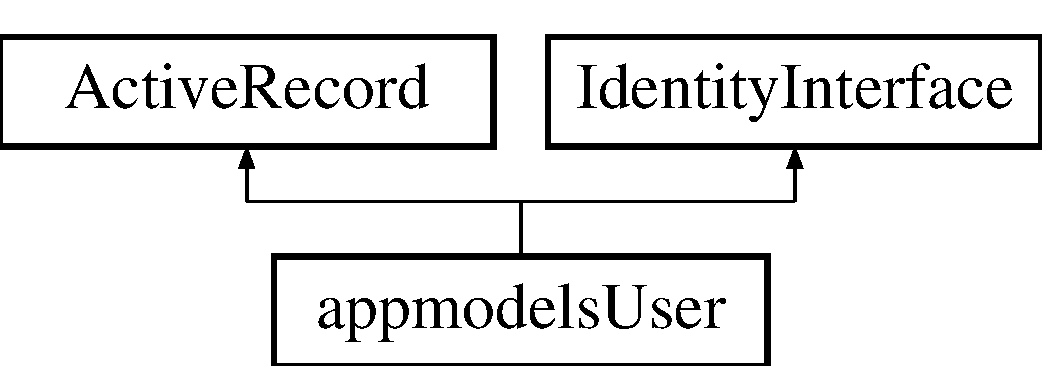
\includegraphics[height=2.000000cm]{classapp_1_1models_1_1User}
\end{center}
\end{figure}
\subsection*{Public Member Functions}
\begin{DoxyCompactItemize}
\item 
\hyperlink{classapp_1_1models_1_1User_a152870bc0603bd20b958f81a59b55cc4}{rules} ()
\item 
\hyperlink{classapp_1_1models_1_1User_a1a34c854f3c6326db1ebf80c5c6c55f0}{attribute\+Labels} ()
\item 
\hyperlink{classapp_1_1models_1_1User_ab78775bd44a0dbca8a40259c7b031cda}{add\+User} (\$model)
\item 
\hyperlink{classapp_1_1models_1_1User_a58f94c4955db10dd3f24e0a99d00586e}{get\+Id} ()
\item 
\hyperlink{classapp_1_1models_1_1User_a5ced30d7fa2a5dce6de833eb8a1d6d0f}{get\+Auth\+Key} ()
\item 
\hyperlink{classapp_1_1models_1_1User_a171ed47858a8b09e7ce70e73a569e304}{validate\+Auth\+Key} (\$auth\+\_\+key)
\item 
\hyperlink{classapp_1_1models_1_1User_a67d493691bfdc5908a43d7aa768bfb6e}{validate\+Password} (\$password)
\end{DoxyCompactItemize}
\subsection*{Static Public Member Functions}
\begin{DoxyCompactItemize}
\item 
static \hyperlink{classapp_1_1models_1_1User_afda20f0337d04f8ef5111dba15462aed}{table\+Name} ()
\item 
static \hyperlink{classapp_1_1models_1_1User_a25abf1d39633efd5d88a36c714f47ea5}{find\+Identity} (\$id)
\item 
static \hyperlink{classapp_1_1models_1_1User_a84e64540978468a276f7d715e1a9ab58}{find\+Identity\+By\+Access\+Token} (\$token, \$type=null)
\item 
static \hyperlink{classapp_1_1models_1_1User_a0a0594e710a25106fcb110132c9b6f83}{find\+By\+Username} (\$username)
\end{DoxyCompactItemize}


\subsection{Member Function Documentation}
\index{app\+::models\+::\+User@{app\+::models\+::\+User}!add\+User@{add\+User}}
\index{add\+User@{add\+User}!app\+::models\+::\+User@{app\+::models\+::\+User}}
\subsubsection[{\texorpdfstring{add\+User(\$model)}{addUser($model)}}]{\setlength{\rightskip}{0pt plus 5cm}app\textbackslash{}models\textbackslash{}\+User\+::add\+User (
\begin{DoxyParamCaption}
\item[{}]{\$model}
\end{DoxyParamCaption}
)}\hypertarget{classapp_1_1models_1_1User_ab78775bd44a0dbca8a40259c7b031cda}{}\label{classapp_1_1models_1_1User_ab78775bd44a0dbca8a40259c7b031cda}
Add a new user to the database 
\begin{DoxyParams}{Parameters}
{\em \hyperlink{classapp_1_1models_1_1SignupForm}{Signup\+Form}} & return Boolean\+: true if insertion succeed, otherwise, false. \\
\hline
\end{DoxyParams}
\index{app\+::models\+::\+User@{app\+::models\+::\+User}!attribute\+Labels@{attribute\+Labels}}
\index{attribute\+Labels@{attribute\+Labels}!app\+::models\+::\+User@{app\+::models\+::\+User}}
\subsubsection[{\texorpdfstring{attribute\+Labels()}{attributeLabels()}}]{\setlength{\rightskip}{0pt plus 5cm}app\textbackslash{}models\textbackslash{}\+User\+::attribute\+Labels (
\begin{DoxyParamCaption}
{}
\end{DoxyParamCaption}
)}\hypertarget{classapp_1_1models_1_1User_a1a34c854f3c6326db1ebf80c5c6c55f0}{}\label{classapp_1_1models_1_1User_a1a34c854f3c6326db1ebf80c5c6c55f0}
\index{app\+::models\+::\+User@{app\+::models\+::\+User}!find\+By\+Username@{find\+By\+Username}}
\index{find\+By\+Username@{find\+By\+Username}!app\+::models\+::\+User@{app\+::models\+::\+User}}
\subsubsection[{\texorpdfstring{find\+By\+Username(\$username)}{findByUsername($username)}}]{\setlength{\rightskip}{0pt plus 5cm}static app\textbackslash{}models\textbackslash{}\+User\+::find\+By\+Username (
\begin{DoxyParamCaption}
\item[{}]{\$username}
\end{DoxyParamCaption}
)\hspace{0.3cm}{\ttfamily [static]}}\hypertarget{classapp_1_1models_1_1User_a0a0594e710a25106fcb110132c9b6f83}{}\label{classapp_1_1models_1_1User_a0a0594e710a25106fcb110132c9b6f83}
Finds user by username


\begin{DoxyParams}{Parameters}
{\em \$username} & string \\
\hline
\end{DoxyParams}
\begin{DoxyReturn}{Returns}
static$\vert$null 
\end{DoxyReturn}
\index{app\+::models\+::\+User@{app\+::models\+::\+User}!find\+Identity@{find\+Identity}}
\index{find\+Identity@{find\+Identity}!app\+::models\+::\+User@{app\+::models\+::\+User}}
\subsubsection[{\texorpdfstring{find\+Identity(\$id)}{findIdentity($id)}}]{\setlength{\rightskip}{0pt plus 5cm}static app\textbackslash{}models\textbackslash{}\+User\+::find\+Identity (
\begin{DoxyParamCaption}
\item[{}]{\$id}
\end{DoxyParamCaption}
)\hspace{0.3cm}{\ttfamily [static]}}\hypertarget{classapp_1_1models_1_1User_a25abf1d39633efd5d88a36c714f47ea5}{}\label{classapp_1_1models_1_1User_a25abf1d39633efd5d88a36c714f47ea5}
\index{app\+::models\+::\+User@{app\+::models\+::\+User}!find\+Identity\+By\+Access\+Token@{find\+Identity\+By\+Access\+Token}}
\index{find\+Identity\+By\+Access\+Token@{find\+Identity\+By\+Access\+Token}!app\+::models\+::\+User@{app\+::models\+::\+User}}
\subsubsection[{\texorpdfstring{find\+Identity\+By\+Access\+Token(\$token, \$type=null)}{findIdentityByAccessToken($token, $type=null)}}]{\setlength{\rightskip}{0pt plus 5cm}static app\textbackslash{}models\textbackslash{}\+User\+::find\+Identity\+By\+Access\+Token (
\begin{DoxyParamCaption}
\item[{}]{\$token, }
\item[{}]{\$type = {\ttfamily null}}
\end{DoxyParamCaption}
)\hspace{0.3cm}{\ttfamily [static]}}\hypertarget{classapp_1_1models_1_1User_a84e64540978468a276f7d715e1a9ab58}{}\label{classapp_1_1models_1_1User_a84e64540978468a276f7d715e1a9ab58}
\index{app\+::models\+::\+User@{app\+::models\+::\+User}!get\+Auth\+Key@{get\+Auth\+Key}}
\index{get\+Auth\+Key@{get\+Auth\+Key}!app\+::models\+::\+User@{app\+::models\+::\+User}}
\subsubsection[{\texorpdfstring{get\+Auth\+Key()}{getAuthKey()}}]{\setlength{\rightskip}{0pt plus 5cm}app\textbackslash{}models\textbackslash{}\+User\+::get\+Auth\+Key (
\begin{DoxyParamCaption}
{}
\end{DoxyParamCaption}
)}\hypertarget{classapp_1_1models_1_1User_a5ced30d7fa2a5dce6de833eb8a1d6d0f}{}\label{classapp_1_1models_1_1User_a5ced30d7fa2a5dce6de833eb8a1d6d0f}
\index{app\+::models\+::\+User@{app\+::models\+::\+User}!get\+Id@{get\+Id}}
\index{get\+Id@{get\+Id}!app\+::models\+::\+User@{app\+::models\+::\+User}}
\subsubsection[{\texorpdfstring{get\+Id()}{getId()}}]{\setlength{\rightskip}{0pt plus 5cm}app\textbackslash{}models\textbackslash{}\+User\+::get\+Id (
\begin{DoxyParamCaption}
{}
\end{DoxyParamCaption}
)}\hypertarget{classapp_1_1models_1_1User_a58f94c4955db10dd3f24e0a99d00586e}{}\label{classapp_1_1models_1_1User_a58f94c4955db10dd3f24e0a99d00586e}
\index{app\+::models\+::\+User@{app\+::models\+::\+User}!rules@{rules}}
\index{rules@{rules}!app\+::models\+::\+User@{app\+::models\+::\+User}}
\subsubsection[{\texorpdfstring{rules()}{rules()}}]{\setlength{\rightskip}{0pt plus 5cm}app\textbackslash{}models\textbackslash{}\+User\+::rules (
\begin{DoxyParamCaption}
{}
\end{DoxyParamCaption}
)}\hypertarget{classapp_1_1models_1_1User_a152870bc0603bd20b958f81a59b55cc4}{}\label{classapp_1_1models_1_1User_a152870bc0603bd20b958f81a59b55cc4}
\index{app\+::models\+::\+User@{app\+::models\+::\+User}!table\+Name@{table\+Name}}
\index{table\+Name@{table\+Name}!app\+::models\+::\+User@{app\+::models\+::\+User}}
\subsubsection[{\texorpdfstring{table\+Name()}{tableName()}}]{\setlength{\rightskip}{0pt plus 5cm}static app\textbackslash{}models\textbackslash{}\+User\+::table\+Name (
\begin{DoxyParamCaption}
{}
\end{DoxyParamCaption}
)\hspace{0.3cm}{\ttfamily [static]}}\hypertarget{classapp_1_1models_1_1User_afda20f0337d04f8ef5111dba15462aed}{}\label{classapp_1_1models_1_1User_afda20f0337d04f8ef5111dba15462aed}
\index{app\+::models\+::\+User@{app\+::models\+::\+User}!validate\+Auth\+Key@{validate\+Auth\+Key}}
\index{validate\+Auth\+Key@{validate\+Auth\+Key}!app\+::models\+::\+User@{app\+::models\+::\+User}}
\subsubsection[{\texorpdfstring{validate\+Auth\+Key(\$auth\+\_\+key)}{validateAuthKey($auth_key)}}]{\setlength{\rightskip}{0pt plus 5cm}app\textbackslash{}models\textbackslash{}\+User\+::validate\+Auth\+Key (
\begin{DoxyParamCaption}
\item[{}]{\$auth\+\_\+key}
\end{DoxyParamCaption}
)}\hypertarget{classapp_1_1models_1_1User_a171ed47858a8b09e7ce70e73a569e304}{}\label{classapp_1_1models_1_1User_a171ed47858a8b09e7ce70e73a569e304}
\index{app\+::models\+::\+User@{app\+::models\+::\+User}!validate\+Password@{validate\+Password}}
\index{validate\+Password@{validate\+Password}!app\+::models\+::\+User@{app\+::models\+::\+User}}
\subsubsection[{\texorpdfstring{validate\+Password(\$password)}{validatePassword($password)}}]{\setlength{\rightskip}{0pt plus 5cm}app\textbackslash{}models\textbackslash{}\+User\+::validate\+Password (
\begin{DoxyParamCaption}
\item[{}]{\$password}
\end{DoxyParamCaption}
)}\hypertarget{classapp_1_1models_1_1User_a67d493691bfdc5908a43d7aa768bfb6e}{}\label{classapp_1_1models_1_1User_a67d493691bfdc5908a43d7aa768bfb6e}
Validates password


\begin{DoxyParams}{Parameters}
{\em \$password} & string password to validate \\
\hline
\end{DoxyParams}
\begin{DoxyReturn}{Returns}
boolean if password provided is valid for current user 
\end{DoxyReturn}


The documentation for this class was generated from the following file\+:\begin{DoxyCompactItemize}
\item 
models/User.\+php\end{DoxyCompactItemize}

\hypertarget{classapp_1_1models_1_1Users}{}\section{app\textbackslash{}models\textbackslash{}Users Class Reference}
\label{classapp_1_1models_1_1Users}\index{app\textbackslash{}models\textbackslash{}\+Users@{app\textbackslash{}models\textbackslash{}\+Users}}
Inheritance diagram for app\textbackslash{}models\textbackslash{}Users\+:\begin{figure}[H]
\begin{center}
\leavevmode
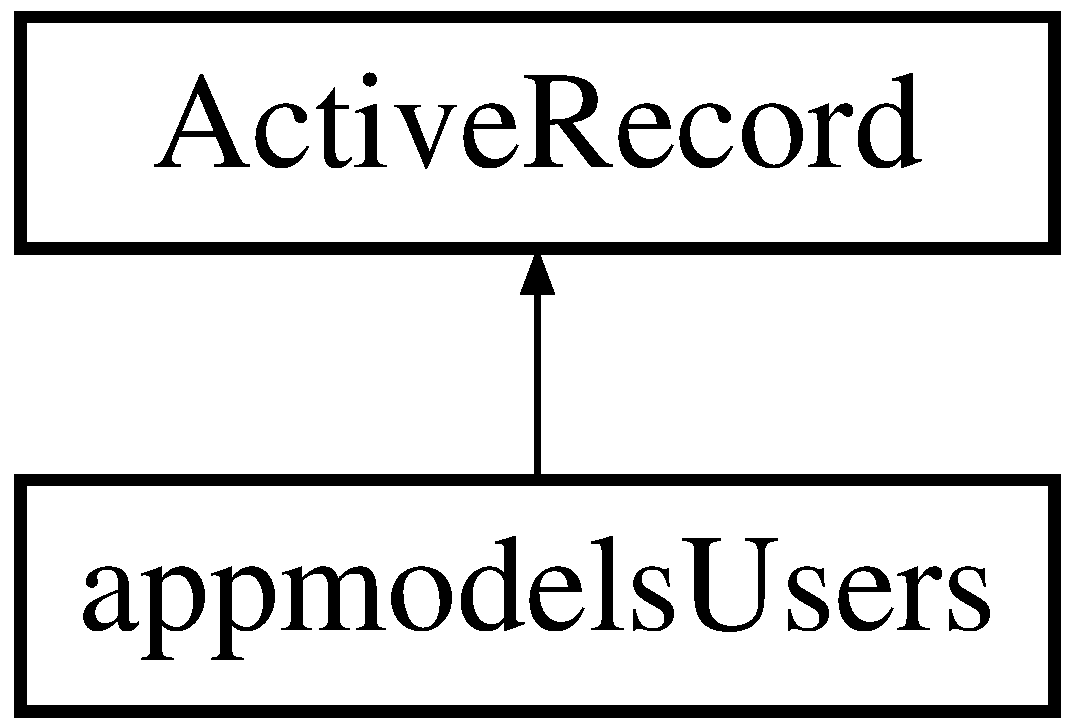
\includegraphics[height=2.000000cm]{classapp_1_1models_1_1Users}
\end{center}
\end{figure}
\subsection*{Public Member Functions}
\begin{DoxyCompactItemize}
\item 
\hyperlink{classapp_1_1models_1_1Users_a83dc33a3554a561f97754c7d8b590c93}{rules} ()
\item 
\hyperlink{classapp_1_1models_1_1Users_ac749ee5c770c8bd22a5cdb4420dccf3a}{attribute\+Labels} ()
\end{DoxyCompactItemize}
\subsection*{Static Public Member Functions}
\begin{DoxyCompactItemize}
\item 
static \hyperlink{classapp_1_1models_1_1Users_a67c4be8e96b91beac8479f378a71785e}{table\+Name} ()
\end{DoxyCompactItemize}


\subsection{Member Function Documentation}
\index{app\+::models\+::\+Users@{app\+::models\+::\+Users}!attribute\+Labels@{attribute\+Labels}}
\index{attribute\+Labels@{attribute\+Labels}!app\+::models\+::\+Users@{app\+::models\+::\+Users}}
\subsubsection[{\texorpdfstring{attribute\+Labels()}{attributeLabels()}}]{\setlength{\rightskip}{0pt plus 5cm}app\textbackslash{}models\textbackslash{}\+Users\+::attribute\+Labels (
\begin{DoxyParamCaption}
{}
\end{DoxyParamCaption}
)}\hypertarget{classapp_1_1models_1_1Users_ac749ee5c770c8bd22a5cdb4420dccf3a}{}\label{classapp_1_1models_1_1Users_ac749ee5c770c8bd22a5cdb4420dccf3a}
\index{app\+::models\+::\+Users@{app\+::models\+::\+Users}!rules@{rules}}
\index{rules@{rules}!app\+::models\+::\+Users@{app\+::models\+::\+Users}}
\subsubsection[{\texorpdfstring{rules()}{rules()}}]{\setlength{\rightskip}{0pt plus 5cm}app\textbackslash{}models\textbackslash{}\+Users\+::rules (
\begin{DoxyParamCaption}
{}
\end{DoxyParamCaption}
)}\hypertarget{classapp_1_1models_1_1Users_a83dc33a3554a561f97754c7d8b590c93}{}\label{classapp_1_1models_1_1Users_a83dc33a3554a561f97754c7d8b590c93}
\index{app\+::models\+::\+Users@{app\+::models\+::\+Users}!table\+Name@{table\+Name}}
\index{table\+Name@{table\+Name}!app\+::models\+::\+Users@{app\+::models\+::\+Users}}
\subsubsection[{\texorpdfstring{table\+Name()}{tableName()}}]{\setlength{\rightskip}{0pt plus 5cm}static app\textbackslash{}models\textbackslash{}\+Users\+::table\+Name (
\begin{DoxyParamCaption}
{}
\end{DoxyParamCaption}
)\hspace{0.3cm}{\ttfamily [static]}}\hypertarget{classapp_1_1models_1_1Users_a67c4be8e96b91beac8479f378a71785e}{}\label{classapp_1_1models_1_1Users_a67c4be8e96b91beac8479f378a71785e}


The documentation for this class was generated from the following file\+:\begin{DoxyCompactItemize}
\item 
models/Users.\+php\end{DoxyCompactItemize}

%--- End generated contents ---

% Index
\backmatter
\newpage
\phantomsection
\clearemptydoublepage
\addcontentsline{toc}{chapter}{Index}
\printindex

\end{document}
